\section{Slackline learning techniques}\label{3_3_learningTechniques}
Section \textit{\nameref{2_1_1_slacklineTraining}} showed that systematic help is not essentially necessary to learn slacklining. The user of the interactive learning system should therefore be able to learn it by herself without any further external help. Therefore section \textit{\nameref{3_3_1_learningConcepts}} differentiates between two learning concepts on which the interactive learning system relies.
%Two learning concepts will be differentiated in subsection \textit{\nameref{3_3_1_learningConcepts}} to achieve this.
Further section \textit{\nameref{3_3_2_StagesExercises}} describes the categorization of specific slackline exercises in the system, which structures at the same time the learning flow of the user.

\subsection{Methods for slackline skill acquisition}\label{3_3_1_learningConcepts}
\subsubsection{Methodical routine}
A methodical routine can be integrated in almost every sport activity. It consists of a series of exercises, whose difficulty increases with further practice. The selected exercises should base on methodical principals that can be scaled by e.g. easy to difficult, known to unknown, or simple to complex~\cite{Fetz1996-ml}. Größing~\cite{Groessing1997-sp} describes the general procedure as follows: at the beginning of a methodical routine the trainee will perform warm up exercises. This is useful to prepare her for the training. After that preliminary exercise will be provided, which are more specific regarding the actual exercises. With this she will learn the general motoric basics and train the movements needed to perform the activity. Further it ensures a smooth transition for the main exercises.

Thomann~\cite{Thomann2013-aa} designed a methodical routine as well as a dynamical methodic for slacklining skill acquisition. His methodical routine inherits various approaches with different elements to reach the goal of learning slacklining. However the integration of these elements are more strict to guide the trainee through a constructive exercise procedure (Figure~\ref{fig:3_3_1_methodicalRoutine}). At first an introduction and preliminary exercises can be integrated. This follows by material and security where the lines dynamic, how to jump off, and controlling of the line is covered. Further the learning of the oscillation behaviour should be implemented with or without methodical help. Afterwards the user can decide to execute balance training with or without help. With help the trainee can directly balance on the line, which includes external support. Without any further help she can decide to first sit, step on the line, or balance independently. Continuing the trainee can decide if she wants to train the static or dynamic balance, which follows by the possibility for more variable exercise execution like walking forwards on the line, walking backwards, with eye closed, etc. Before going to train some tricks on the line, which is on the very end of the routine, the trainee has to learn first staying across the line with her feet. This is a necessary part for several tricks and has to be learned before.
\begin{figure}[htb]
	\centering
	\begin{minipage}[t]{1\linewidth}
		\centering
		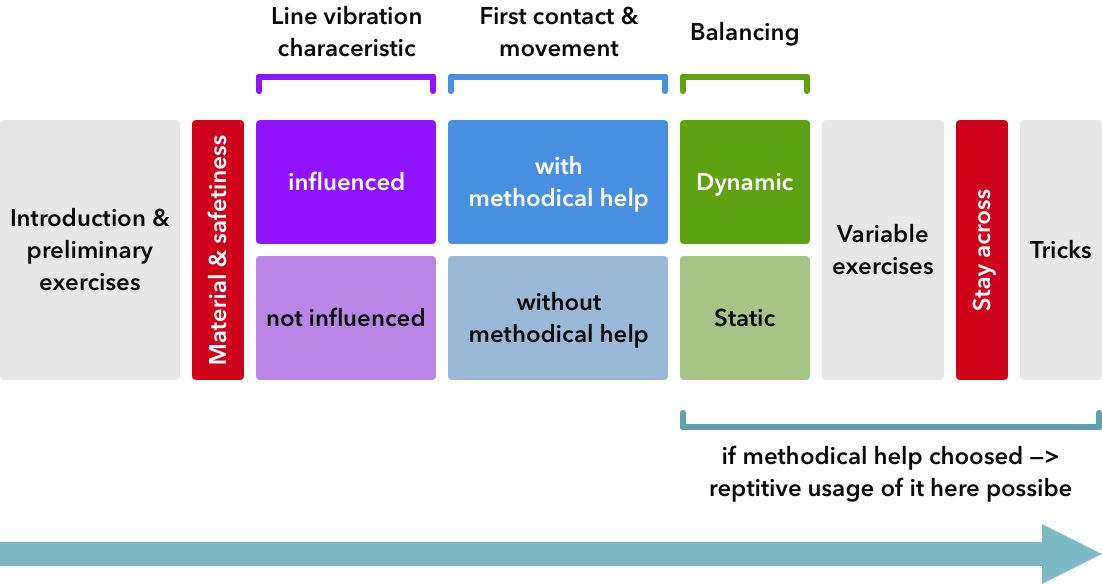
\includegraphics[width=1\linewidth]{Pictures/3_3_1_methodicalRoutine3}
		\caption{Methodical routine~\cite{Thomann2013-aa}}
		\label{fig:3_3_1_methodicalRoutine}
	\end{minipage}
\end{figure}

\subsubsection{Differential methodic}
The differential or dynamic methodic follows another approach. It is in coherence with an open learning situation~\cite{Thomann2013-aa}. This means it depends on several factors, which in slacklining would be line type and length, tension, environment, etc. Considering the interplay of these factors each trainee can construct her own training set. A dynamic methodic is a practical usage for this~\cite{Beck2008-dl, Schoellhorn1999-ip}. This inherits the model of stepping stones. In general it describes that many possibilities can lead to the same goal. Each potential way has therefore its own difficulty level. This results in a more modular way to reach a specific goal. In comparison to the methodical routine it results in bigger differences in stimulus and provide more variability in the movement execution, like compared in figure~\ref{fig:3_3_1_comparisonMethods}. 

\begin{figure}[htb]
	\centering
	\begin{minipage}[t]{1\linewidth}
		\centering
		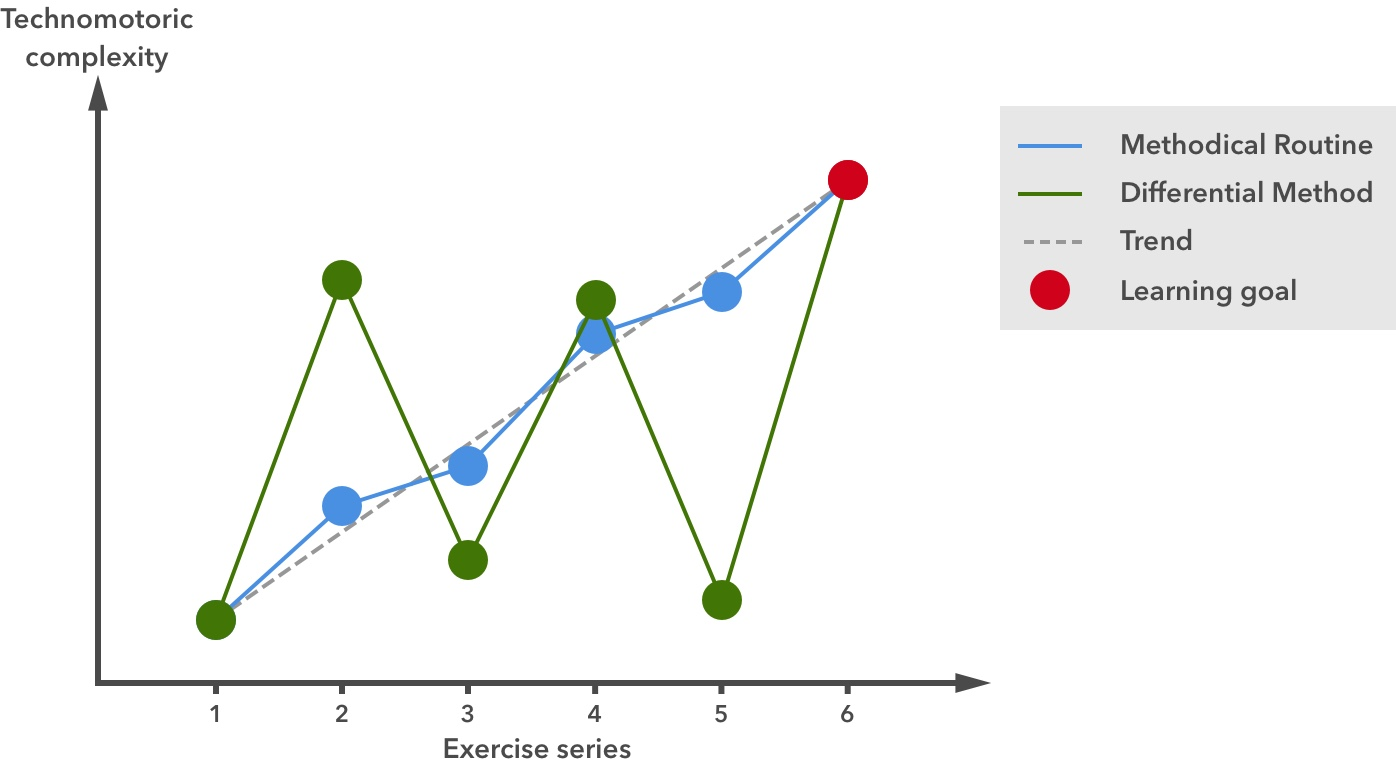
\includegraphics[width=0.83\linewidth]{Pictures/3_3_1_comparisonMethod2}
		\caption{Comparison methodical routine vs. differential method~\cite{Thomann2013-aa}}
		\label{fig:3_3_1_comparisonMethods}
	\end{minipage}
\end{figure}
To make us of the principle of differential learning the trainee can follow a methodical principle like seen in methodical routine. If she reaches a certain threshold of skill level more dynamic procedures can then be involved in the actual learn process. %Therefore the principle of differential learning can be used, which results in big stimulus differences and provide more variability in the movement execution.

The usage in slacklining can be integrated like described and visualized by Thomann~\cite{Thomann2013-aa} (Figure \ref{fig:3_3_1_dynamicMethod}). He divided exercises into five learning stages an in its coordinative demand and complexity. The main goal is to master controlled and complex movements on the line. The trainee has to choose an amount of various exercise of all stages. Each more complex exercise can either be supported by methodical help or the trainee can return to the lower stage to learn the movement for the specific exercise. Each trainee can therefore create her individual path. Modification and integration of more useful exercises are allowed. Structured examples can be seen in figure~\ref{fig:3_3_1_dynamicMethod}. The purple arrows visualize a way for people that are more coordinative, more venturesome, or have background knowledge. In contrast the green arrows visualize a path for people that are less coordinate, less venturesome, or have no background knowledge in slacklining.

\begin{figure}[htb]
	\centering
	\begin{minipage}[t]{1\linewidth}
		\centering
		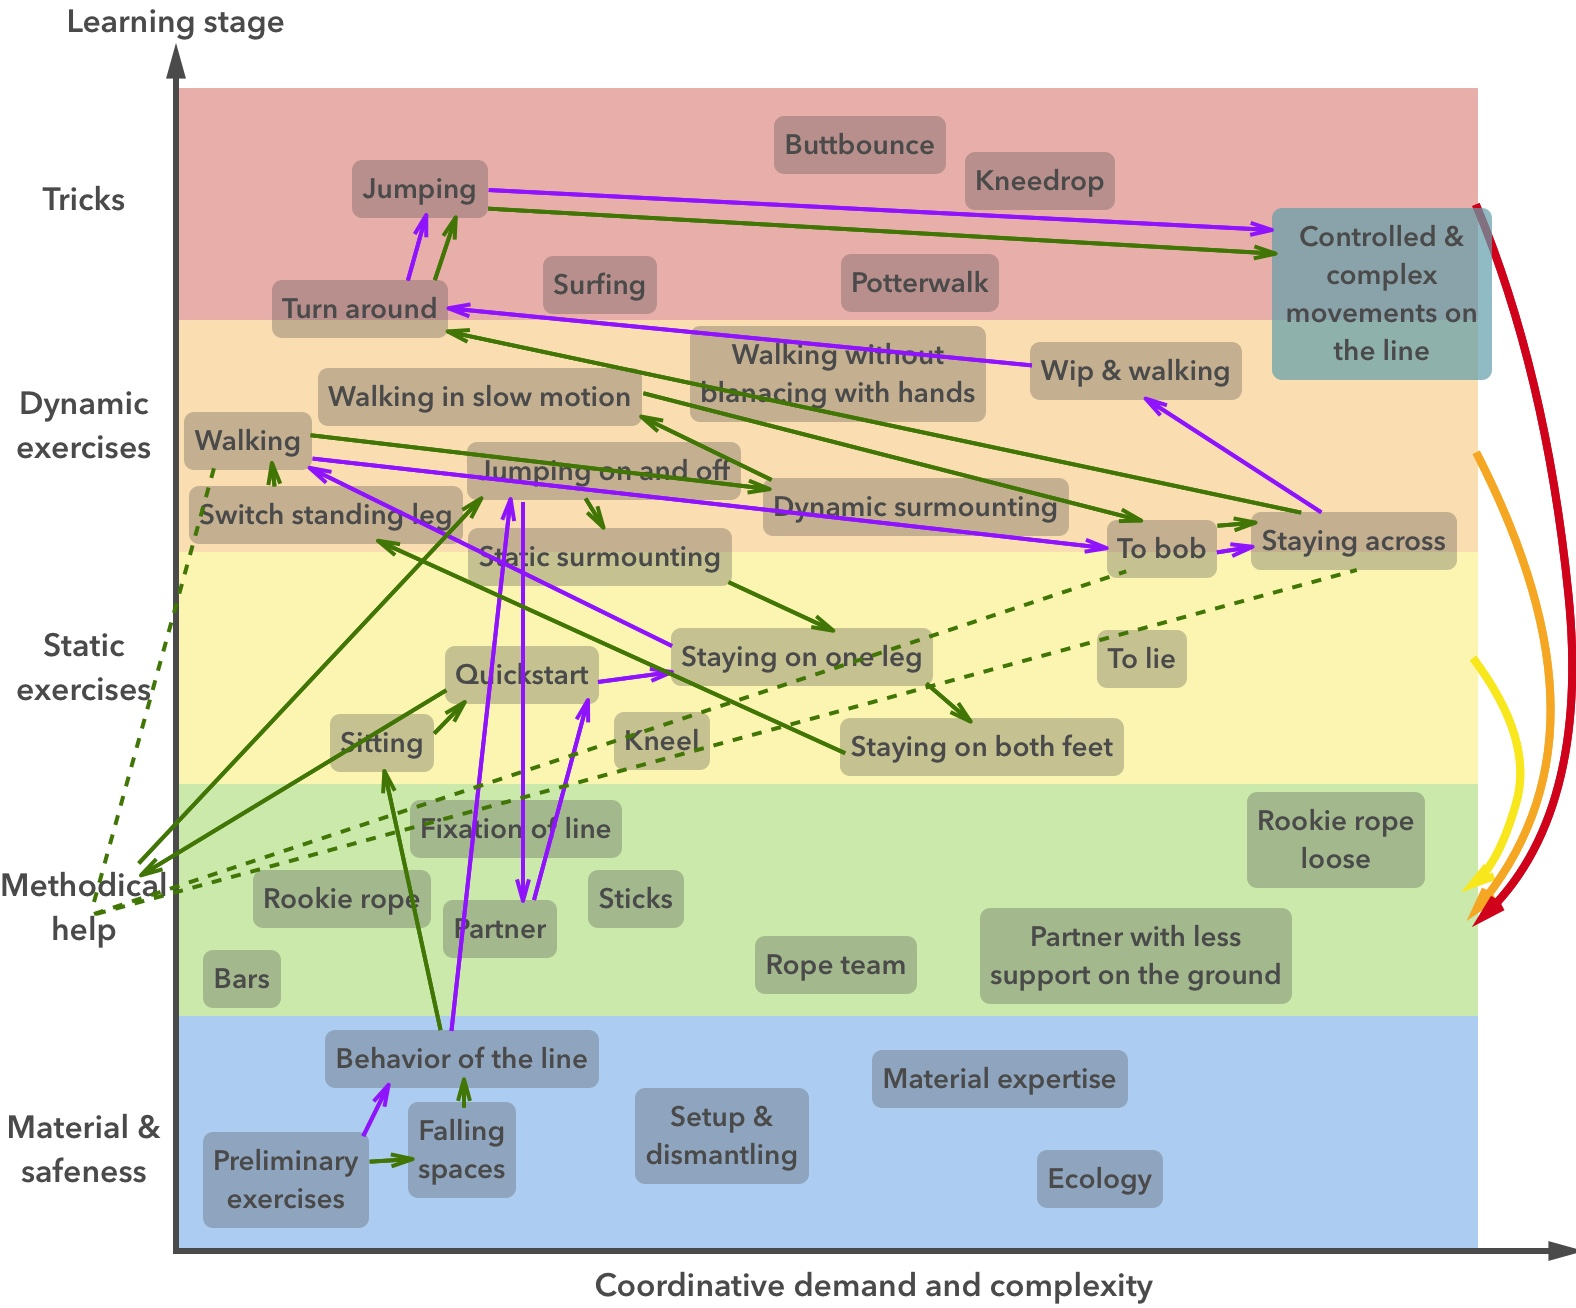
\includegraphics[width=1\linewidth]{Pictures/3_3_1_dynamicMethod3}
		\caption{Dynamic methodic in slacklining~\cite{Thomann2013-aa}}
		\label{fig:3_3_1_dynamicMethod}
	\end{minipage}
\end{figure}

For proper user training with the system the trainee should follow a clear workflow. Therefore the methodical routine is the better choice as a learning concept in this interactive learning system. She learns right from the beginning essential aspects of slacklining that are relevant and build up on each other. Because it follows a strict linear sequence stages and exercises can be designed as levels. 
%The trainee can unlock further levels by successfully executing the prior exercise. 
The next subsection \textit{\nameref{3_3_2_StagesExercises}} will therefore cover a clear workflow integration of exercises for this learning system.

\subsection{Stages and exercise of learning slacklining}\label{3_3_2_StagesExercises}
% Drei verschiedene Grundfertigkeiten: zunächst muss man auf einem Bein stehen können, dazu kommt die schmale Unterstützungsfläche, auf der man balancieren soll. Nicht zuletzt befindet man sich in einer gewissen Höhe und nicht mehr auf sicherem Boden.
Now that an overview about slacklining and its learning techniques are given several practical exercises have to be considered. Repetitive trials are one approach of learning to walk on the line. However this could result in dangerous situations and frustration of the slacker because of her missing skills. Therefore an exercise set is elaborated that teach and guide the slacker. The teaching goal should be that the slacker can balance with a controlled manner on the line, stay on it for a few seconds, and be able to walk a few steps. In general one has to acquire three core skills to achieve this goal~\cite{Kroiss2007-ab}. At first the slacker should be able to stay on one foot. This is essential because most of the time the slacker has a standing foot on the line and the other one servers as balance component. Second the balancing on a narrow surface since the slackline exists of a limited width. Lastly managing the height is also important due to the fact that the slackline is mostly tensed around the knee height and above.

As a groundwork the elaborated exercises are based on Kroiß~\cite{Kroiss2007-ab}. He elicited learning exercises for beginners on a slackline within a school class, which gives a good basic on the exercise integration. Further several other references~\cite{Balcom2005-wl, Donath2013-kk, Donath2016-gm, Granacher2010-ow, Keller2012-xh, Kleindl2011-bl, Pfusterschmied2013-yy, Thomann2013-aa} have been researched to elaborate exercises that fit the best in this system. Each exercise is therefore categorized in one of four tiers, which represent the fundamental basis of the exercises routine. In the following each tier is introduced, its goal clarified, and the learning aspects described:

\subsubsection{Tier I - Preliminary exercises}
The first tier serves as a preparation for the subsequent exercises. Hence just exercises on the ground will be executed. This is to train and strengthen the persons general physical balance. In general it is recommended to train barefoot or with socks to get a better foot feeling. The knees should be bent to have a better initial position for movement compensation. Keeping the head up and setting a focus point can help to calm the visual sense of balance. In almost all exercises of this tier the arms have to be stretched to the side, be over the shoulder, and bent in about 135 degree. This is the biggest balance function overall because you have freedom in all directions and the slacker can shift her body's center of gravity. Further all exercises should be executed slowly and controlled to master the body behaviour.

\subsubsection{Tier II - First contact with the line}
Mastering the general physical balancing leads the slacker to her first experience with the slackline. The goal is to get a feeling for the slackline and to be able to get up on the line as well as hold herself for a short amount of time. For this the slacker has to become familiar with the line, feel the imbalance, how her body wants to behave, and get a feeling for counterbalancing unpredictable movements. Therefore starting at the sweet spot, that's about 1/3 of the line, can help. It's an area with a comfortable vibration characteristic. The foot should also be always in alignment with the slackline to have the biggest amount of surface of your foot covered with the line, which results in more contact area of the foot. If the slacker has problems with holding her hands over the shoulder, she can turn the palms to the top and the hands will then raise automatically up. A relaxed but straight upper body can help to hold the right position.

\subsubsection{Tier III - Static exercises}
More difficult exercises come in this tier. The slacker is now familiar with the line and able to stand for a short amount of time on it. The goal is that the slacker should stay confidently on the line. Further it serves as preparation for walking on the line. All prior learned techniques have to be directly applied. The non standing leg now comes more into action. It serves as an additional balancing parameter to both of the arms. If the slacker has problems with going up on the line, she can keep the balancing leg vertically in line with the standing leg while going up and then move it to the side. The pressure is mostly around the ball of the foot.

\subsubsection{Tier IV - Dynamic exercises}
This is the last tier and it involves the dynamical part for the slackline. The slacker should now be able to stay confidently on the line with one foot and both feet. The goal is to learn how to make the first steps as a result for walking on the line. In general it is applying static exercises together. While staying on the line and when the slacker wants to make a step she can guide her balancing foot to the side of the line and shift it then forwards. Letting the knees together when making a step forward helps because the legs can support each other. Making small steps won't shift the body's center of gravity that much forward, which results in more control.
